\chapter{Inferring Human Actions and Intentions} % Main chapter title

\label{chapter:intention} % Change X to a consecutive number; for referencing this chapter elsewhere, use \ref{ChapterX}

\lhead{Chapter 3. \emph{Intention Recognition}} % Change X to a consecutive number; this is for the header on each page - perhaps a shortened title

In this chapter we show how our system is able to infer human actions and intentions. Section~\ref{sec:intention-intro} introduces the problem of intention recognition, discussing some related studies. Section~\ref{sec:intention-intention_recognition} shows our approach at solving this problem, while section~\ref{sec:intention-proactive_behaviors} discusses the proactive behaviors that the robot can execute after inferring the human's intention.  Finally, section~\ref{sec:intention-example} shows an example of a run of our algorithm.


\section{Introduction}
\label{sec:intention-intro}
A crucial skill to interact with humans is recognizing others' actions and goals. This process is is directly linked to modeling humans' beliefs, since, as explained by \cite{byom2013theory} ``as humans, we generally believe that others act in ways that are consistent with their beliefs and goals". 

The recognition of human activities is an important topic in computer science research, which can be studied at different levels. Anticipating human actions and movements allows the robot to adapt its behavior and proactively help humans, as studied in \cite{koppula2013anticipating}. 

Sequences of actions can be linked to plans, a well-known topic called plan recognition. Several approaches have been studied in this domain using, for example, classical planning \citep{ramirez2009plan}, probabilistic \citep{bui2003general} or logic techniques \citep{singla2011abductive}.

As previously said, we call an intention the wish and will to achieve a goal. Intention recognition is intrinsically linked to plan recognition, since, if an agent is acting by following a plan we can assume that it has the intention of achieving a goal. In the rest of this chapter, we will consider plan recognition as a way to recognize intentions. 

Other approaches that can be used to estimate the intention of a human are Interactive Partially Observed Markov Decision Processes (I-POMDP) and Inverse Learning. I-POMDP~\citep{gmytrasiewicz2004interactive} offer a rich framework that extends Partially Observed Markov Decision Processes (POMDP) in a multi-agent setting. Inference in these models can be extremely complex, but there have been attempts at solving this issue, like in~\cite{doshi2009monte,hoang2013interactive}. 

Inverse Reinforcement Learning~\citep{ng2000algorithms} formulates the problem of computing an unknown reward function of an agent after observing his behavior. This strategy has been applied, with Bayesian Networks (BN), in~\cite{Nagai2015}, in order to learn the mental model of another agent, and choose appropriate actions for a relationship building task. A linked approach is inverted planning, which has been applied in a bayesian framework in~\cite{baker2009action}  for human action understanding.

Contextual information can be used to further disambiguate complex situations. For example, if it is currently raining (context), we could think that it is more likely that Greg will look for his umbrella (intention) if he has to go out. ~\cite{Liu2014} show a system using BNs to understand users' intentions with an emphasis on contextual information. This BN is constructed using object affordance nodes (e.g. a cup can be washed or used for drinking), context nodes (e.g. it's a hot day, the cup was recently used), and intention nodes (e.g. drinking from a cup or washing it). The causal links between contexts and intentions are learnt through a user study, which uses an online questionnaire where participants need to rate the strenght of the connection betwen an intention and a context. The work does not study how to adapt this BN to complex plans, composed by sequences of actions.

It is very important to consider humans' beliefs when estimating their intentions. In a dynamic environment, agents can execute actions, modifying the state of the world without other agents being able to perceive the changes. Let us imagine a scenario. Bob comes back home from work and would like to relax while reading. He lays down on a sofa with a book, and reaches to a nearby table to grab his glasses. He does not know that his wife, during the day, moved the glasses to another room. If we would ignore Bob's beliefs on the world (i.e. he does not know that the glasses are not on the table) we could infer that, for example, Bob would like a drink while he is sitting on the sofa, or the tv remote controller. If, instead, we would know that Bob thinks his glasses are on the table (and we would use other contextual information perhaps, like Bob's habitudes) we would be able to correctly infer Bob's current intention, that is, taking his glasses, and warn him that they are not there, perhaps even fetching them for him. 

In robotics, an interesting framework that considers this issue is the Bayesian Theory of Mind \citep{baker2014modeling}, used to represent the inference process of an observer looking at another agent's behaviors. The acting agent is modeled as a POMDP, whose richness is able to represent his possible beliefs about the world. The observer's process is modeled as a DBN, built starting from the agent's POMDP but considering his reward function (that represents his desires) as hidden. The system has been tested against some alternative models and compared, in user studies, with human capacities, to understand how well it models theory of mind. Since the models used are quite complex, scalability in the model could be an issue. Also, the study is focused on a single-agent scenario, and does not consider collaborative problems.

Let us examine the two simulation-based systems that we already presented in the previous section, HAMMER~\citep{demiris2007prediction}, and the architecture of \cite{BreazealGB09}, and see how these cognitive architectures are able to infer actions and intentions.

The HAMMER system is organized with couples of inverse and forward models.  Inverse models receive as input the goal and state of the system, producing the motor commands which are needed to achieve the goal. Forward models, instead, receive as input motor commands and compute the predicted future state. When these two models are linked, the forward model receives as input the motor commands produced by an inverse model. This link can form a loop, with the output of a forward model returning to its inverse model, which can adjust a range of parameters if the predicted future state does not match exactly the desired state. These models can be organized in parallel schemas and used to recognize actions performed by a demonstrator. 

In this case, the demonstrator's current state, as perceived by the robot, is fed in the inverse models, which in turn send their output to the forward models. The state predicted by the forward models are compared with the demonstrator's state at the next time step. This comparison produces a score, which can be used to infer the most likely action performed. 

Forward and inverse models can be organized in hierarchical schemas, to infer tasks and plans. The complexity of these schemas could be quite significant, particularly when trying to recognize a goal which can be achieved in many different ways, depending on the context. 

\cite{BreazealGB09} uses a similar ideas, where all the possible robot movements are represented as a graph of connected poses, with arcs showing possible transitions between the poses. This graph is used both to represent the robot's movements and to map observed trajectories. Tasks are represented as schemas, which can be organized in sequential and hierarchical structures to model complex goals.

 When trying to infer an agent's intention, the robot looks for a schema whose motor action matches the observed activities of the agent. After that, the schema is traversed in reverse in order to try to determine the real intention. The system is not able to deal with ambiguities, and this algorithm stops if it comes to a point where there is more than a possible explanation for the current behavior. 

An example of non simulation-based system in this topic is \cite{talamadupula2014coordination}. This architecture is used to coordinate human-robot teams, based on intention recognition and belief modeling. Creating and maintaining beliefs is handled using the strategy explained in~\cite{scheutz2013computational}, presented in the previous chapter. Prediction of other humans' intentions is based on the plan recognition algorithm of ~\cite{ramirez2009plan}. While this algorithm uses efficient replanning to increase its efficiency, in complex domains, where the users have many different strategies to achieve a goal, the system would need to execute frequent replans to infer the actual strategy chosen by the user, which can be expensive.

Our goal was developing an algorithm able, through inference, to recognize human actions and connect them to possible intentions. To avoid errors in interpretation, we decided to use humans' belief models, and not the robot knowledge, to perform our reasonings. We also decided to use contextual information to further disambiguate our estimation. Another goal was to make this algorithm fast and scalable. 

This algorithm was introduced in~\cite{devin2016some} and we will show, in the next sections, how it was designed. 

\section{Intention and Action Inference}
\label{sec:intention-intention_recognition}
In order to infer actions and intentions, we will provide the following information to the robot: a list of known contexts, a list of known intentions, a list of known actions, a set of observations of human actions, and belief model of humans and of the robot itself.

We introduce a simplification in our model: at each time step, a human can execute only one action and has only one intention, decreasing the ambiguities in the inference process.

We propose, as central model used for intention estimation, a framework based on BNs. We call our implementation of BN an Intention Graph (IG).
An IG is linked to a specific human, and composed by the following layers of nodes:
\begin{itemize}
\item Context Nodes: these nodes represent contextual information, modeled as boolean variables (e.g. HotDay, ColdDay).
\item Intention Nodes: these boolean nodes represent the set of possible intentions. Each intention can depend on several contexts.
\item Action Nodes. This is the set of human actions whose preconditions are satisfied in the human's mental belief when the IG is created. Each of these nodes is dependent on all the intention nodes. 
\item Observation Nodes. We associate to each action a different set of observation nodes, that depend on the associated action node. For example, the distance of a human from the \textit{target} of an action can be an Observation Node.
\end{itemize}

In a typical usage, the robot will create, for each monitored human, an IG, formed by the Context and Intention Nodes, which we consider statically known by the robot, and a variable list of Action and Observation nodes, which depends on the human's belief model. The robot will create action nodes for each known action whose $preconditions$ are \textit{satisfied in the human's belief model}, and their related Observation Nodes. We stress, in particular, that actions are created based on the human's belief model, since the human might be trying to execute actions that are actually impossible in the current situation (e.g. the human tries to take an object from a basket without looking inside it. He does not know that the object is not there anymore).  These IGs will be updated every time that an agent performs an action, creating and removing Action and Observation nodes, depending on the state of the world after the action was performed.

When monitoring a human, we set Context Nodes and Observation Nodes as \textit{evidence}, considering them observable by the robot. These information will allow us to have a good estimation of the most likely actions and intentions of the human, as explained in subsection~\ref{sec:intention-intention and action inference}. 

An example of IG, taken from an experiment, can be seen in figure~\ref{fig:intention-intention_graph}. In the following paragraphs, we will explain the role of these layers of nodes, and how the conditional dependencies between them are computed.  After that, we will show, in section~\ref{sec:intention-example}, an example showing how an IG is created and updated following a sequence of human actions, and how the robot is able to use it to infer the most likely human intention.

 \begin{figure}[ht!]
	\centering
	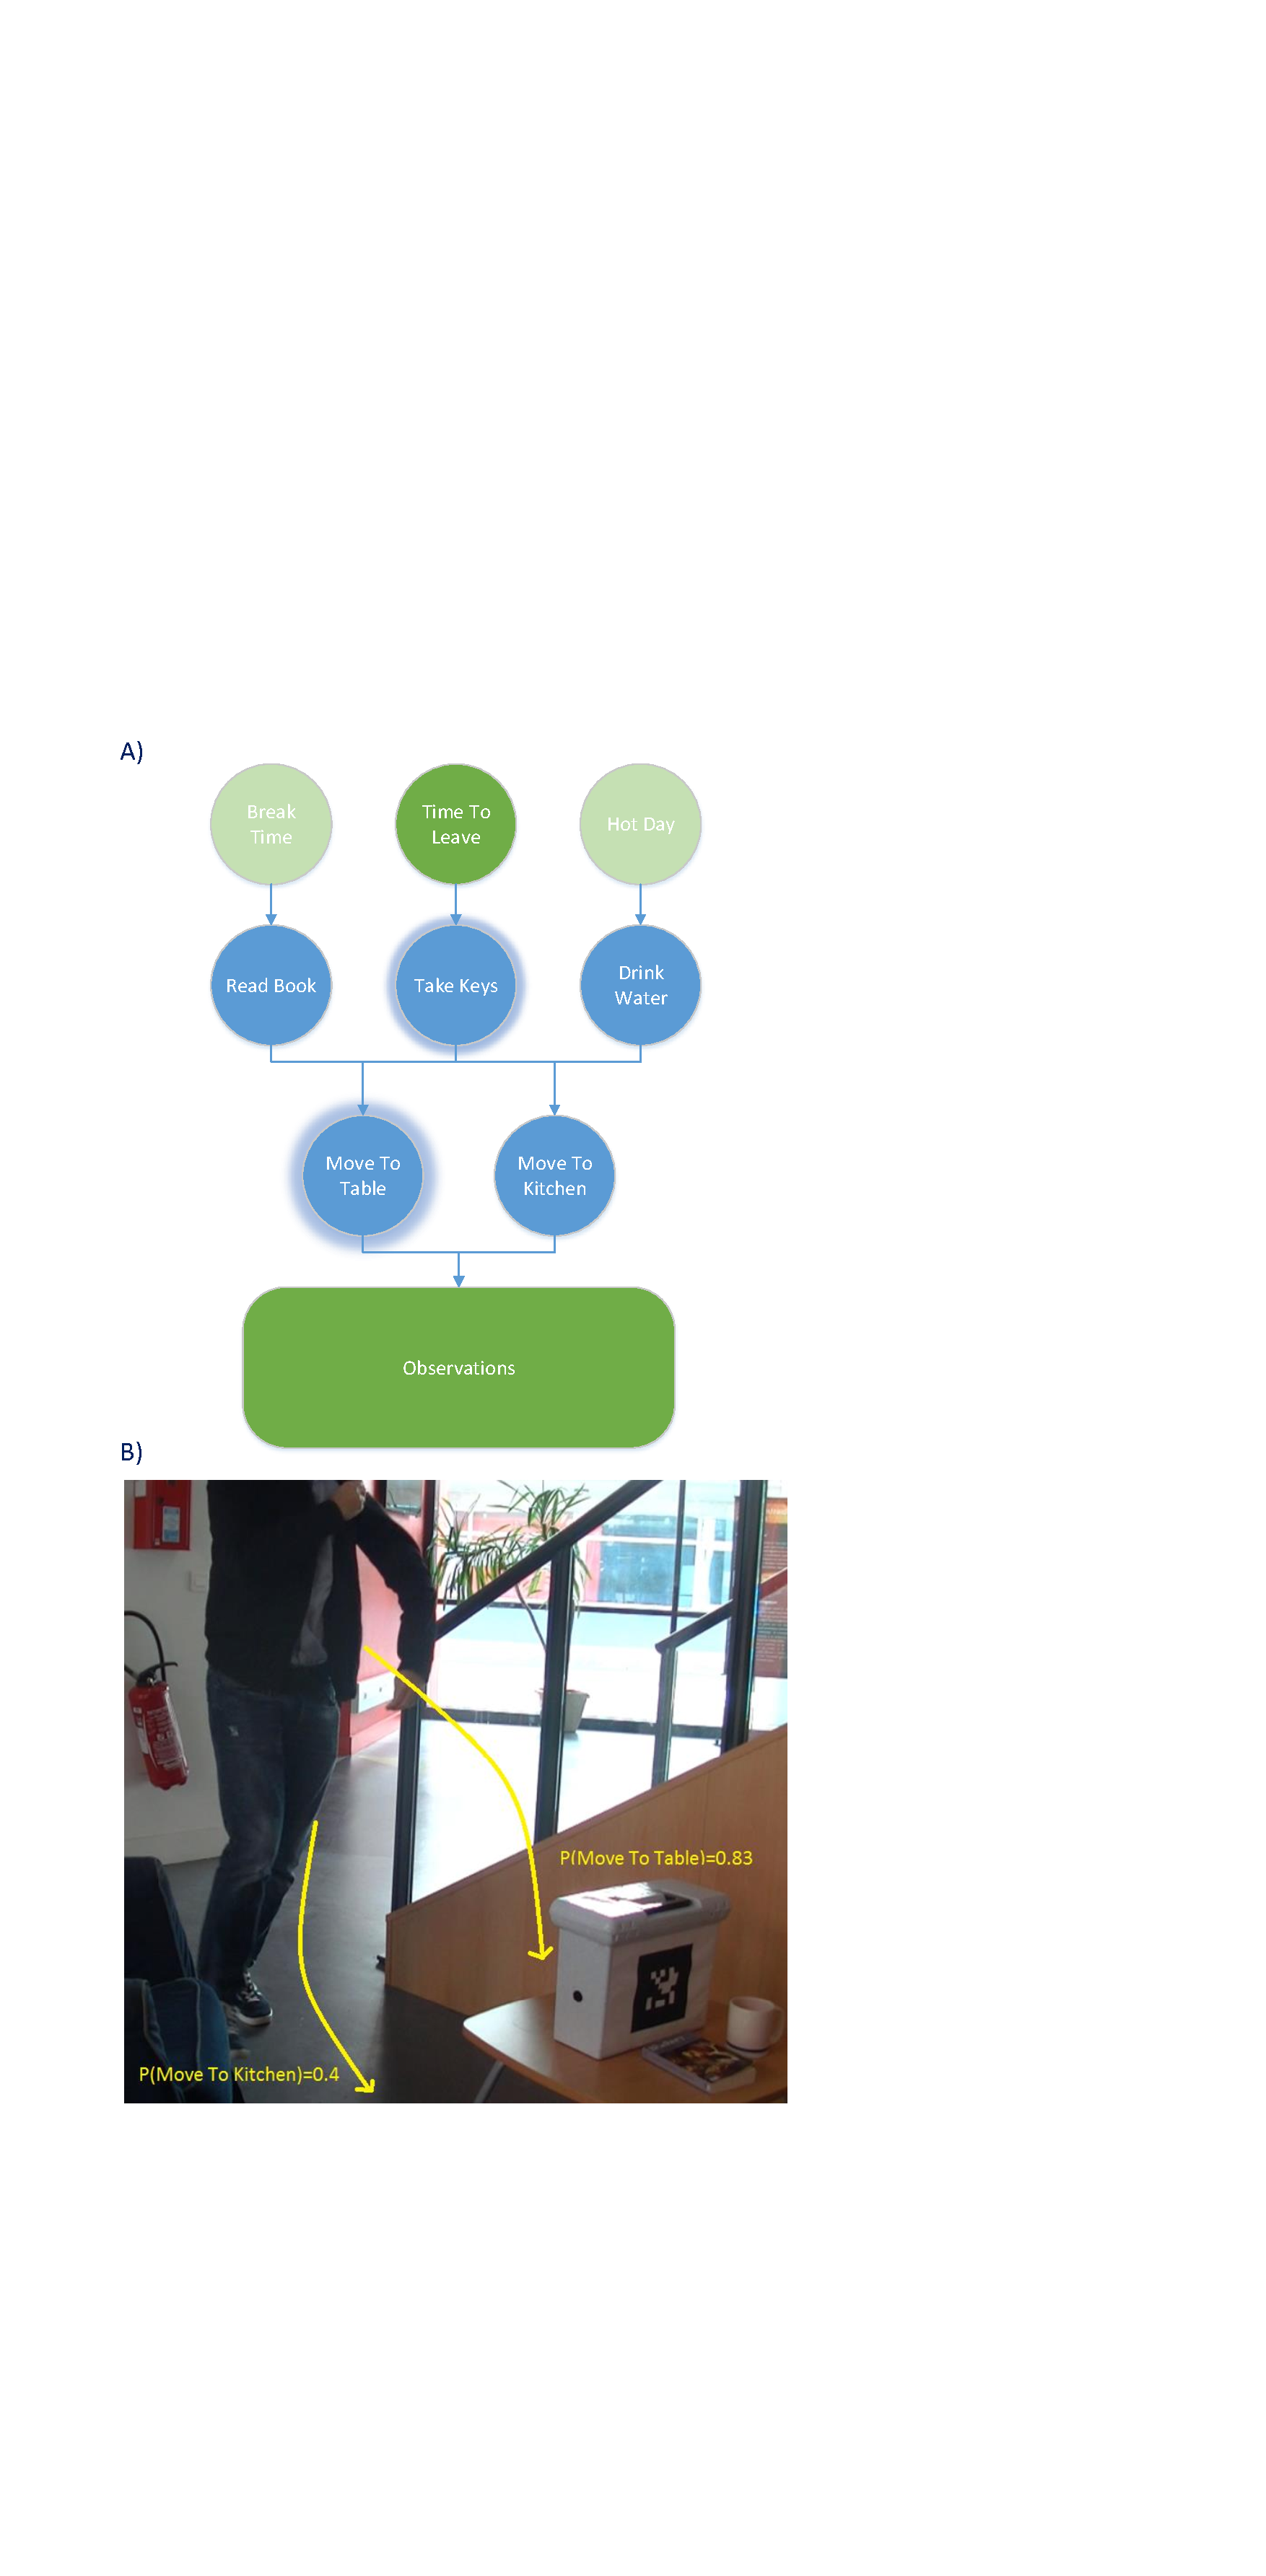
\includegraphics[trim={2cm 11cm 11cm 17cm},clip,scale=0.45]{img/observer/cookieScenario.pdf}
	\caption[Intention Graph]{A scene from our experiment. The yellow arrows show possible actions and their associated probabilities. The diagram represents the current IG. Green circles represent evidence nodes and blue circles other nodes. For the Context Nodes (top of the graph), we represented nodes with a false value as greyed out, and nodes with a true value as green. The most likely nodes in the graph are represented with a glowing effect. The observation nodes were compressed in a single block to simplify the diagram}
	\label{fig:intention-intention_graph}
\end{figure}


\subsection{From Contexts to Intentions}
We introduce a set of contexts in our domain. We consider as context any information that can be used to characterize and motivate an intention \citep{abowd1999towards}. We model a context  as a fact, which can assume different values and influences the probability of a user having a particular intention. For example, we imagine that a human is more likely to be cooking at dinner time, or to drink a hot mug of tea on a cold day.

Contextual nodes can directly influence one or more Intention Nodes. In this work, we chose to learn these conditional dependencies from humans, as explained in subsection~\ref{subsec:observer_results-system_implementation}.

\subsection{From Intentions to Actions}
\label{sec:intention-action_evaluation}
To understand how actions are linked to intentions the robot needs to answer the following question: what actions would a human take, in this situation, given his belief of the world, in order to achieve its intention?
Our idea is based on the principle of rationality \citep{Dennet1989}, which states that agents tend to choose the most efficient actions, taking into account their beliefs about the world, in order to achieve their desires.

In~\cite{Blakemore2001}, the authors explain that ``the attribution of intentions to actions might rely on simulating the observed action and mapping it into representations of our own intention". We represent this idea by providing the robot with a set of planning models. Each one of these planning models is related to an intention, and represents all the known plans to achieve its linked goal. In this way, we can estimate how much the current human actions are compatible with the plans related to an intention.

In our implementation, for each intention known by the robot, we will create an associated Markov Decision Process (MDP), to represent all the possible plans linked to this intention. After solving the set of MDPs we will use the calculated action value function \(Q(s,a)\), to create conditional dependencies between Intention and Action Nodes in the IG. We define \(P(a|I_i=1)\), the probability that action $a$ will be performed if intention $I_i$ is true, as as:
\begin{equation}
 P(a|I_i=1)=\frac{Q_i(s,a)}{\sum_b(Q_i(s,b))}
\end{equation}
  where we normalize the value function $Q_i(s,a)$ for intention $i$ and action $a$ in the human's belief state $s$, over the value function $Q_i(s,b)$ calculated on all the monitored actions $b$. 

%   We can extend this calculation to the case where a generic number of intentions are true to compute the probabilities of action nodes: 
% \begin{equation}
%   P(a|I_1,I_2,...,I_m)=\frac{\sum_{i:I_i=1}Q_i(s,a)}{\sum_b\sum_{i:I_i=1}Q_i(s,b)}
% \end{equation}

The key idea in this problem is to use the human's belief state as input for the MDPs' value functions. In this way we are using perspective taking at a planning level, since the human action will be consistent with his intention in his own belief state but may be not optimal, irrelevant, or even dangerous in the real world (e.g. in case of wrong belief).

Our idea is similar to \cite{karami2010human}. In this work, the robot planning model is a POMDP, where the human intention is a hidden variable. The transition function for the human intention is computed starting from the action values obtained from a set of human MDPs, that simulate human policies related to different intentions. In this work, we used a BN for the inference process, instead of a POMDP. This allows us to include in a simple way more information in the inference process, such as context, and to separate the mechanisms used for inference and for the robot's actions. Also, we improve the recognition process by including the belief state of the human.

\subsection{From Actions to Observations}
Intentions will be inferred from human actions, so the robot needs to monitor their execution. For each Action Node we can define a different set of Observation Nodes, which depend on the specific actions. Typical examples are: the distance of the human's body from the action's $target$, its variation, the distance of the human's hand from the action's $target$, and its variation. The conditional dependencies of the Observation Nodes are precomputed.

\subsection{Intention and Action Inference}
\label{sec:intention-intention and action inference}
We assume, in this work, that at each moment a human can only execute a single action, and the robot will react only to his most likely intention. The most likely action and intention are inferred from the BN in the following way. We call $P(n)$ the inferred probability of a node $n$, $B(n)$ the set of brothers of $n$ (that is, nodes on the same layer), and $\delta_1$, $\delta_2$ two thresholds. The robot selects the most likely action and intention following these rules: 
\begin{itemize}
\item  \(P(n_i)>\delta_1\) 
\item  \(\forall b \in B(n_i): P(n_i)>P(b)+\delta_2\), where $n_i$ is the node associated to the interested intention or action.
\end{itemize}

To infer that an action has been performed, the robot uses an estimation of the action's probability and geometrical reasoning. For example, the robot infers that a human has taken a bottle if his hand is closer to it than a threshold $\sigma$  and the action's probability in the IG respect the previous rules. For another example, the robot infers that a human has mixed some ingredients in a bowl if his hand approaches the bowl and then leaves after some seconds, always taking into account the probability of the action in the IG.

When the robot infers that an action has been performed, it updates the world state with its $postconditions$, triggering an update on the beliefs of all present agents. The current human intention is recorded in the Database, and will be used by the Goal Management layer.

 \begin{figure}[ht!]
	\centering
	\includegraphics[scale=0.8, trim={0 4cm 0 0}]{img/observer/pick.pdf}
	\caption[Actions and world update]{The human picks an object and the robot updates accordingly the world state. The spheres surrounding objects show when the human's hand is considered to be near an object.}
	\label{fig:intention-pick}
\end{figure}

\subsection{Action Inference with Unknown Intentions}
\label{subsec:intention-unknown_intentions}
In some situations, we are interested in inferring human actions without using information from intentions. When the robot is cooperating with a human, we assume that the human will follow a set of actions to achieve the cooperative goal following a shared plan. The MDPs used in our implementation are able to plan only for a single-agent, and can not be used to represent the shared plan. This could be a problem, because when agents act alone, they might execute different actions than when acting together. For example, if Greg and the robot are reordering a room together, Greg might give the robot a book, because in the shared plan the robot will put it in its place. If Greg is acting alone, he will need to place the book back by himself.  

In this situation, we will create an IG using only actions and observations. In this way, we can still infer which actions are executed, but we have to rely only on geometrical reasoning. Since we are using limited perception algorithms, we could easily encounter ambiguous situation, where, for example, the human moves his hand toward two close objects. In this situation, without using higher level information, the system could make mistakes, and infer that the wrong action has been performed.

We will discuss, in chapter~\ref{chapter:mamdp} about a possible multi-agent MDP implementation to solve this issue.

\section{Proactive Behaviors}
\label{sec:intention-proactive_behaviors}
Information about the most likely intention and action will be introduced in the Situation Assessment layer's Database, to be read by the Goal Management layer. Based on this information, the robot can execute two different proactive behaviors: correcting the belief state of the human, and proactively helping him to achieve his task.

\subsection{Correcting Belief State}
Having a wrong or incomplete belief on the world state can lead agents to execute non optimal, useless, or even dangerous actions. The robot needs to detect these situations in order to warn the human. For example Greg could search for his glasses in a wrong location if he does not know that they were moved, or could touch a hot object if he does not know its temperature.

 The robot assumes that it always holds a correct belief state. Our solution uses the expected action rewards introduced in \ref{sec:intention-action_evaluation}. The idea is comparing the expected reward for performing an action according to the human and the robot's belief states. To formalize: we compare the action values \(Q_m(s_h,a_h)\) and \(Q_m(s_r,a_h)\), where $m$ is the most likely intention,  $s_h$ and $s_r$ are the robot's and human's belief state, and $a_h$ is the most likely action. If these values are not equal the human expects a different outcome from its action than what should actually happen. 

We propose a simple solution, where the robot warns the human of the detected divergent belief for that action. For example, Bob wants to drink tea from a closed, opaque bottle, which the robot knows is empty (perhaps because another agent drank the last glass), while Bob does not. When he approaches the bottle, the robot detects that his most likely intention is to drink tea. 

The system calculates the expected rewards from taking the bottle in the two belief models and obtains different values. The system checks the facts related to the attributes associated to the target of the action (i.e. the bottle) in the two mental models, and extracts the differences.  Using this information, the robot corrects the divergent belief, informing the human that the bottle is now empty. 

If there is no difference in the belief models, it means that the divergent belief is actually related to a future action that the human is expected to execute. For example, let us imagine a scenario where Greg is trying to prepare a dish, requiring pasta and tomatoes. Let us imagine that Greg does not know that there are no more tomatoes, and moves to take the pasta. Using Greg's belief model, there will be a certain reward to take the pasta, since it is a necessary step to prepare the dish. In the robot's belief model, the reward will be zero (assuming that he correctly inferred the intention of Greg to prepare pasta with tomato sauce), because there are no more tomatoes. While there are is no divergent belief on attributes related to the pasta, it would be useful if the robot would inform Greg that there are no more tomatoes.

A solution is extracting an horizon of future actions from the MDP related to the \textit{prepare pasta with tomato sauce} intention. Our system can do this by simulating an update on the MDP, considering as starting state the current human belief model, choosing actions from the agent's policy computed when solving the model, and taking as next states the most likely effects of the actions. We can repeat the reasoning on the targets of each action in this horizon, in order to find a divergent belief. 

If we can still not find a divergent belief, the robot can only inform a human that there might be a problem to achieve its goal, but it is not able to identify it.

% In our system, the Goal Management layer will detect these situations, by reading the Database, and choose a \textit{warn agent} goal (as will be explained in chapter \ref{chapter:goal_management}).

In a real scenarios, the human might have several divergent beliefs at the same time. While the robot could inform the human as soon as it detects a divergent belief, it would risk overloading him with unneeded information. For example, Greg might not know that his wife drank a mug of coffee or moved the remote control to the table, but maybe he will not need these information in the near future. We chose, with this approach, to give information about a divergent belief only when it risks impacting the actions of a human.

\subsection{Performing a part of the plan}
There are situations in which the robot should help the human achieve its goal by physically acting. The Goal Management layer will consider new inferred intentions as possible goals for the robot, and will communicate with the Plan Management layer to achieve them, as explained in chapters~\ref{chapter:plan_management} and~\ref{chapter:task_execution}. 

\section{Intention Graph Example}
\label{sec:intention-example}

\subsection{Scenario}
We will now show an example of use of an IG. We start by defining a scenario with a human, Greg, and two possible intentions: drinking water and reordering a table, by moving all the objects on top of it to the kitchen. We set three different locations: a \textit{table}, a \textit{shelf}, and a \textit{kitchen}. We consider two objects: a \textit{glass} and a \textit{bottle}. Both these objects can contain water, but the \textit{bottle} is opaque and Greg can not observe if there is water or not in it. We simplify the situation by imagining that the bottle is already open. Of course, this scenario is not realistic and is chosen just to illustrate the IG. In a real situation Greg would notice that the bottle is empty when taking it, because it would be too light, or by looking through its hole.

At the start of the scenario, Greg is at the \textit{shelf}, the \textit{bottle} and \textit{glass} are on the \textit{table}, and the they are both empty.  We set a situation of divergent belief, where Greg does not know that the bottle is empty, but the robot has this information. 

We introduce two predicates: \textit{isAt}, that represented the location of an entity, and can assume the values \textit{TABLE}, \textit{SHELF}, and \textit{KITCHEN}; and \textit{capacity}, which indicates if an object contains water, and can assume the values \textit{0} and \textit{1}. 

The belief models of Greg and of the robot are shown in table~\ref{table:intention-ig_bm}, while the set up for this scenario is shown in figure~\ref{fig:intention-ig_scenario}.

 \begin{table}[h!]
\centering
\scriptsize
\renewcommand{\arraystretch}{1.3}
\begin{tabular}{|c|c|}
\hline
Robot & Human \\ \hline \hline
GLASS isAt TABLE  & GLASS isAt TABLE \\ \hline
BOTTLE isAt TABLE & BOTTLE isAt TABLE \\ \hline
GLASS capacity 0  & GLASS capacity 0  \\ \hline
BOTTLE capacity 0 & BOTTLE capacity 1 \\ 
\hline
\end{tabular}
\caption[Belief models in the IG scenario]{Belief models for Greg and for the robot in the IG example scenario. There is a divergent belief situation, where Greg does not know that the bottle is currently empty, represented by the fact \textit{BOTTLE capacity VALUE} }
 \label{table:intention-ig_bm}    
\end{table}



 \begin{figure}[ht!]
	% \centering
	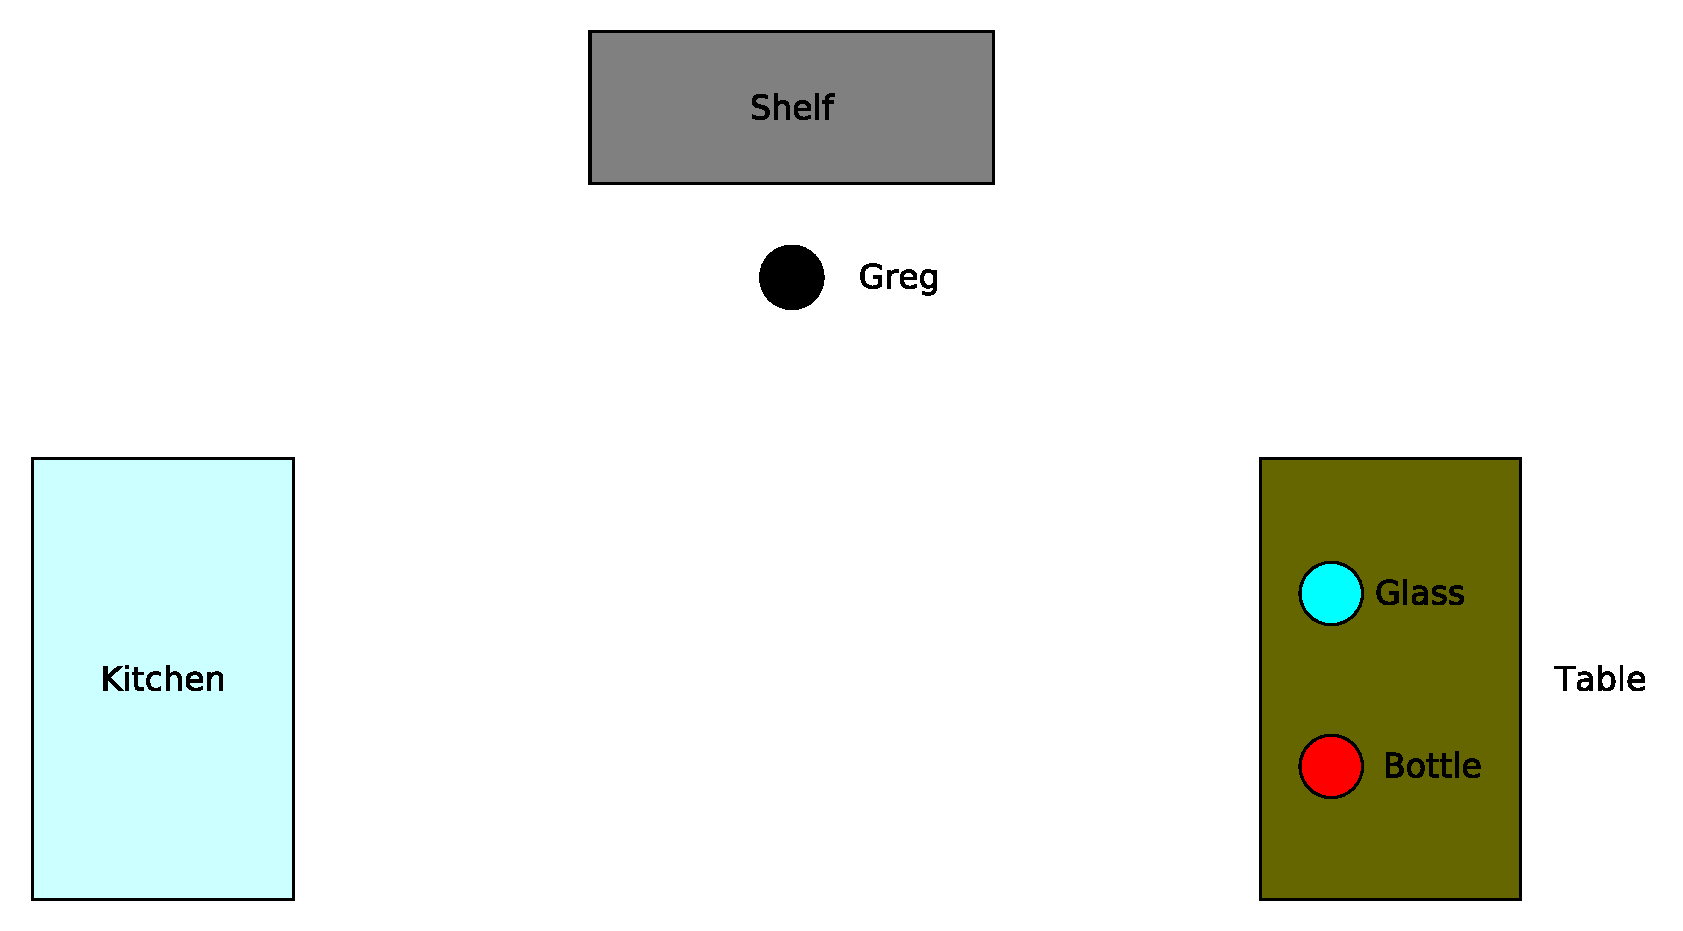
\includegraphics[scale=0.5]{img/observer/ig_scenario.pdf}
	\caption[IG Example Scenario]{The image shows the set-up for the IG example scenario. The locations are represented as different rectangles. Greg is represented as a black circle. The glass and bottle are represented, respectively, by a blue circle and a red circle.}
	\label{fig:intention-ig_scenario}
\end{figure}

We introduce two contexts in the scenario: \textit{HotDay}, representing the fact that the day is particularly warm, and \textit{AlreadyDrank}, representing the fact that the human has recently drank water.

We introduce this possible set of actions in the scenario: taking the bottle, taking the glass, filling the glass using the bottle, drinking from the glass, moving to the kitchen, moving to the table, placing the objects in different locations. We simplify this set to only include the actions relevant to this example, and so we do not include the possibility for Greg to refill the bottle with water. Also, we consider that Greg can only hold a single object at a moment. 

\subsection{Building the Intention Graph}
We build a starting IG with the following nodes:
\begin{itemize}
	\item Context Nodes: \textit{HotDay}, \textit{AlreadyDrank}.
	\item Intention Nodes: \textit{DrinkWater}, \textit{ReorderTable}.
	\item Action Nodes: \textit{MoveTable}, \textit{MoveKitchen}. These two actions are introduced in the IG because they are the only ones whose $preconditions$ are currently satisfied, since Greg can move in any location where he is not at the moment.
	\item Observation Nodes: \textit{BodyDistanceTable}, \textit{TowardTable}, \textit{BodyDistanceKitchen}, \textit{TowardKitchen}. The \textit{BodyDistance} nodes represent the distance between Greg and the target of an action, and can assume the values \textit{close}, \textit{medium}, \textit{far}, \textit{out of range}. The \textit{Toward} nodes are \textit{true} if the distance between \textit{Greg} and the object is decreasing, and false otherwise.
\end{itemize}


In this scenario, we precompute the probability table of the causal links between Context Nodes and Intention Nodes, and between Action Nodes and Observaton Nodes. We set a causal link between \textit{HotDay} and \textit{DrinkWater}, and one between \textit{AlreadyDrank} and \textit{ReorderTable}. In both cases, we use the probability table of table~\ref{table:intention-ig_intention}.

 \begin{table}[h!]
\centering
\begin{tabular}{|c|c|c|}
\hline
Context & \multicolumn{2}{|c|}{Intention} \\ \hline \hline
& 0 & 1 \\ \hline
0  & 0.6 & 0.4 \\ \hline
1 & 0.4 & 0.6 \\ \hline
\end{tabular}
\caption{Conditional probabilities of the Intention Nodes in the IG example scenario.}
 \label{table:intention-ig_intention}    
\end{table}

We consider as slightly more likely that Greg wants to drink water in a Hot Day, and that he wants to reorder the table if he drank recently.

We set a causal link between each action and its observation nodes. For example, \textit{MoveTable} will have a causal link with \textit{BodyDistanceTable} and \textit{TowardTable}. In both actions, we use the probability table of tables~\ref{table:intention-ig_toward} and~\ref{table:intention-ig_distance}.

 \begin{table}[h!]
\centering
\begin{tabular}{|c|c|c|}
\hline
Action & \multicolumn{2}{|c|}{Toward} \\ \hline \hline
& 0 & 1 \\ \hline
0  & 0.8 & 0.2 \\ \hline
1 & 0.2 & 0.8 \\  \hline
\end{tabular}
\caption{Conditional probabilities of the Toward Nodes in the IG example scenario.}
 \label{table:intention-ig_toward}    
\end{table}

 \begin{table}[h!]
\centering
\begin{tabular}{|c|c|c|c|c|}
\hline
Action & \multicolumn{4}{|c|}{Distance} \\ \hline \hline
& Close & Medium & Far & Out of Range \\ \hline
0  & 0.16 & 0.2 & 0.25 & 0.39 \\ \hline
1 & 0.39 & 0.25 & 0.2 & 0.16 \\ \hline
\end{tabular}
\caption{Conditional probabilities of the Distance Nodes in the IG example scenario.}
 \label{table:intention-ig_distance}    
\end{table}

If Greg is executing an action, it  more likely that he is moving toward the action's $target$. For example, the \textit{MoveTable} action is more likely the closer Greg is to the table and if the distance to it is decreasing.

\subsection{Building the Human MDPs}
To set the conditional probabilities between Intention and Action Nodes, we created two different MDPs, each related to one of the intentions. We will now show the state space $S$, action set $A$ and reward function $R$  of the two MDPs. We do not include the transition function of the model as it is extensive and does not help understanding this example.

\begin{itemize}
\item DrinkWater:
\begin{itemize}
\item $S$: $\{agent\_isAt, glass\_isAt, bottle\_isAt, bottle\_capacity, glass\_capacity\}$.
\item $A$: $\{agent\_move\_table, agent\_move\_kitchen, agent\_move\_shelf, agent\_take\_bottle, \\ 
agent\_take\_glass, 
agent\_fill\_glass\_bottle, agent\_drink\_glass, agent\_place\_bottle\_table, \\ agent\_place\_bottle\_kitchen, agent\_place\_bottle\_shelf, agent\_place\_glass\_table, \\ agent\_place\_glass\_kitchen, agent\_place\_glass\_shelf\}$.
\item $R(s,a)=1000 \quad \text{if} \\
glass\_isAt==agent\_isAt \; \text{AND} \; glass\_capacity==1  \; \text{AND} \; a==agent\_drink\_glass$.
\end{itemize}


\item ReorderTable:
\begin{itemize}
\item $S$: $\{agent\_isAt, glass\_isAt, bottle\_isAt\}$.
\item $A$: $\{agent\_move\_table, agent\_move\_kitchen, agent\_move\_shelf, agent\_take\_bottle,\\ agent\_take\_glass, 
agent\_place\_glass\_kitchen, agent\_place\_bottle\_kitchen\}$.
\item $R(s,a)=1000 \quad \text{if} \\
(glass\_isAt==kitchen \; \text{AND} \; bottle\_isAt==human \; \text{AND} \; a==human\_place\_bottle\_kitchen)  \\
 \text{OR} \\
 (glass\_isAt==human \; \text{AND} \; bottle\_isAt==kitchen \; \text{AND} \; a==human\_place\_glass\_kitchen)$.
\end{itemize}
\end{itemize}

After solving these MDPs we used their action value functions to compute the conditional probabilities for the Action Nodes, as shown in section~\ref{sec:intention-action_evaluation}.

\subsection{Simulated Run}
We will now show a simulated run of this scenario in three steps. This run was created by introducing a stream of observations in the system, including the actions that Greg will perform. We consider that Greg's intention in this example is \textit{Drink Water}. We will conduct three different tests for each step:
\begin{itemize}
	\item Test 1. We create the IG using the human's mental belief state to compute the causal links between Action and Intention Nodes. We do not use context to help disambiguate the intentions.
	\item Test 2. We add contextual information to Test 1, setting \textit{HotDay} to \textit{true} and \textit{RecentlyDrank} to \textit{false}.
	\item Test 3. We do not use contextual information and use the robot's mental belief state to compute the causal links between Action and Intention Nodes. This means that the robot will evaluate Greg's action by considering that he knows that the bottle is currently empty (even though he does not know).
\end{itemize}

We will now describe and discuss these stages:
\begin{itemize}
	\item Greg is approaching the \textit{table}, as shown in figure ~\ref{fig:intention-ig_exp1}. The observations are updated correspondingly, and the probabilities of the actions are computed. The action \textit{MoveTable} has the highest probability. 
		\begin{itemize}
			\item Test 1. At this stage, the system is not able to infer the correct intention. Greg could be going to the \textit{table} to take the objects and bring them to the \textit{kitchen} or to drink water. The probability of the two intentions is both 0.50.
			\item Test 2. By using context, the system is already able to infer the correct intention. The probability of \textit{DrinkWater} becomes 0.69, and that of \textit{ReorderTable} 0.3. The robot could already fire a proactive behavior to inform Greg that the \textit{bottle} is, in fact, empty.
			\item Test 3. Without context, the system thinks that Greg is trying to reorder the table, since it is not possible to drink water because the \textit{bottle} is empty. The system would infer a wrong intention.
		\end{itemize}
	\item Greg has arrived to the \textit{table}, as shown in figure~\ref{fig:intention-ig_exp2}. The $postconditions$ of the action are added to the mental models of the robot and of Greg, changing Greg's location. The system creates a new IG, setting as actions those whose $preconditions$ are now satisfied: \textit{MoveKitchen}, \textit{MoveShelf}, \textit{TakeGlass}, and \textit{TakeBottle}. At this point, Greg's hand moves toward the \textit{bottle}, and the observations nodes are set appropriately.
		\begin{itemize}
			\item Test 1. The system is still not able to disambiguate between the two intentions. Greg could be taking the  \textit{bottle} to fill the \textit{glass} or to bring it to the \textit{kitchen}.
			\item Test 2. In this case, the context is still providing the missing information to understand that Greg wants to drink water.
			\item Test 3. In this case, since it is not possible to drink water in the robot's mental belief, the system is still inferring the wrong intention.
		\end{itemize} 
	\item Greg has taken the \textit{bottle}, and is now bringing it to the \textit{glass}, as shown in figure~\ref{fig:intention-ig_exp3}. A new IG is created, containing the actions that are now executable: \textit{MoveKitchen}, \textit{MoveShelf}, \textit{PlaceBottleTable}, and \textit{FillGlass}. In test 3, the IG created would not contain the action to fill the glass with water, since it is not executable in the robot's mental belief model, where the \textit{bottle} is empty.
		\begin{itemize}
			\item Test 1. At this point, the system has enough information to understand that Greg's intention is \textit{DrinkWater}, which assumes a probability of 0.90. The system can now fire a proactive behavior, with the robot informing Greg of the divergent belief. Even though the actions \textit{PlaceBottleTable} and \textit{FillGlass} could be ambiguous from a geometric point of view (since, in both cases, the arm of the human will approach the table), the system infers that the action performed was \textit{FillGlass} since it is more \textit{useful} in the current situation and with the considered intentions.
			\item Test 2. Context confirms this intention, bringing the probability to 0.95.
			\item Test 3. In this case, Greg's movement would not be understood, since in the robot's mental belief model it is not possible to fill the glass with water. Greg's action would actually be inferred as \textit{PlaceBottleTable}, which has no use for any intention.
		\end{itemize}
\end{itemize}

 \begin{figure}[ht!]
	\centering
	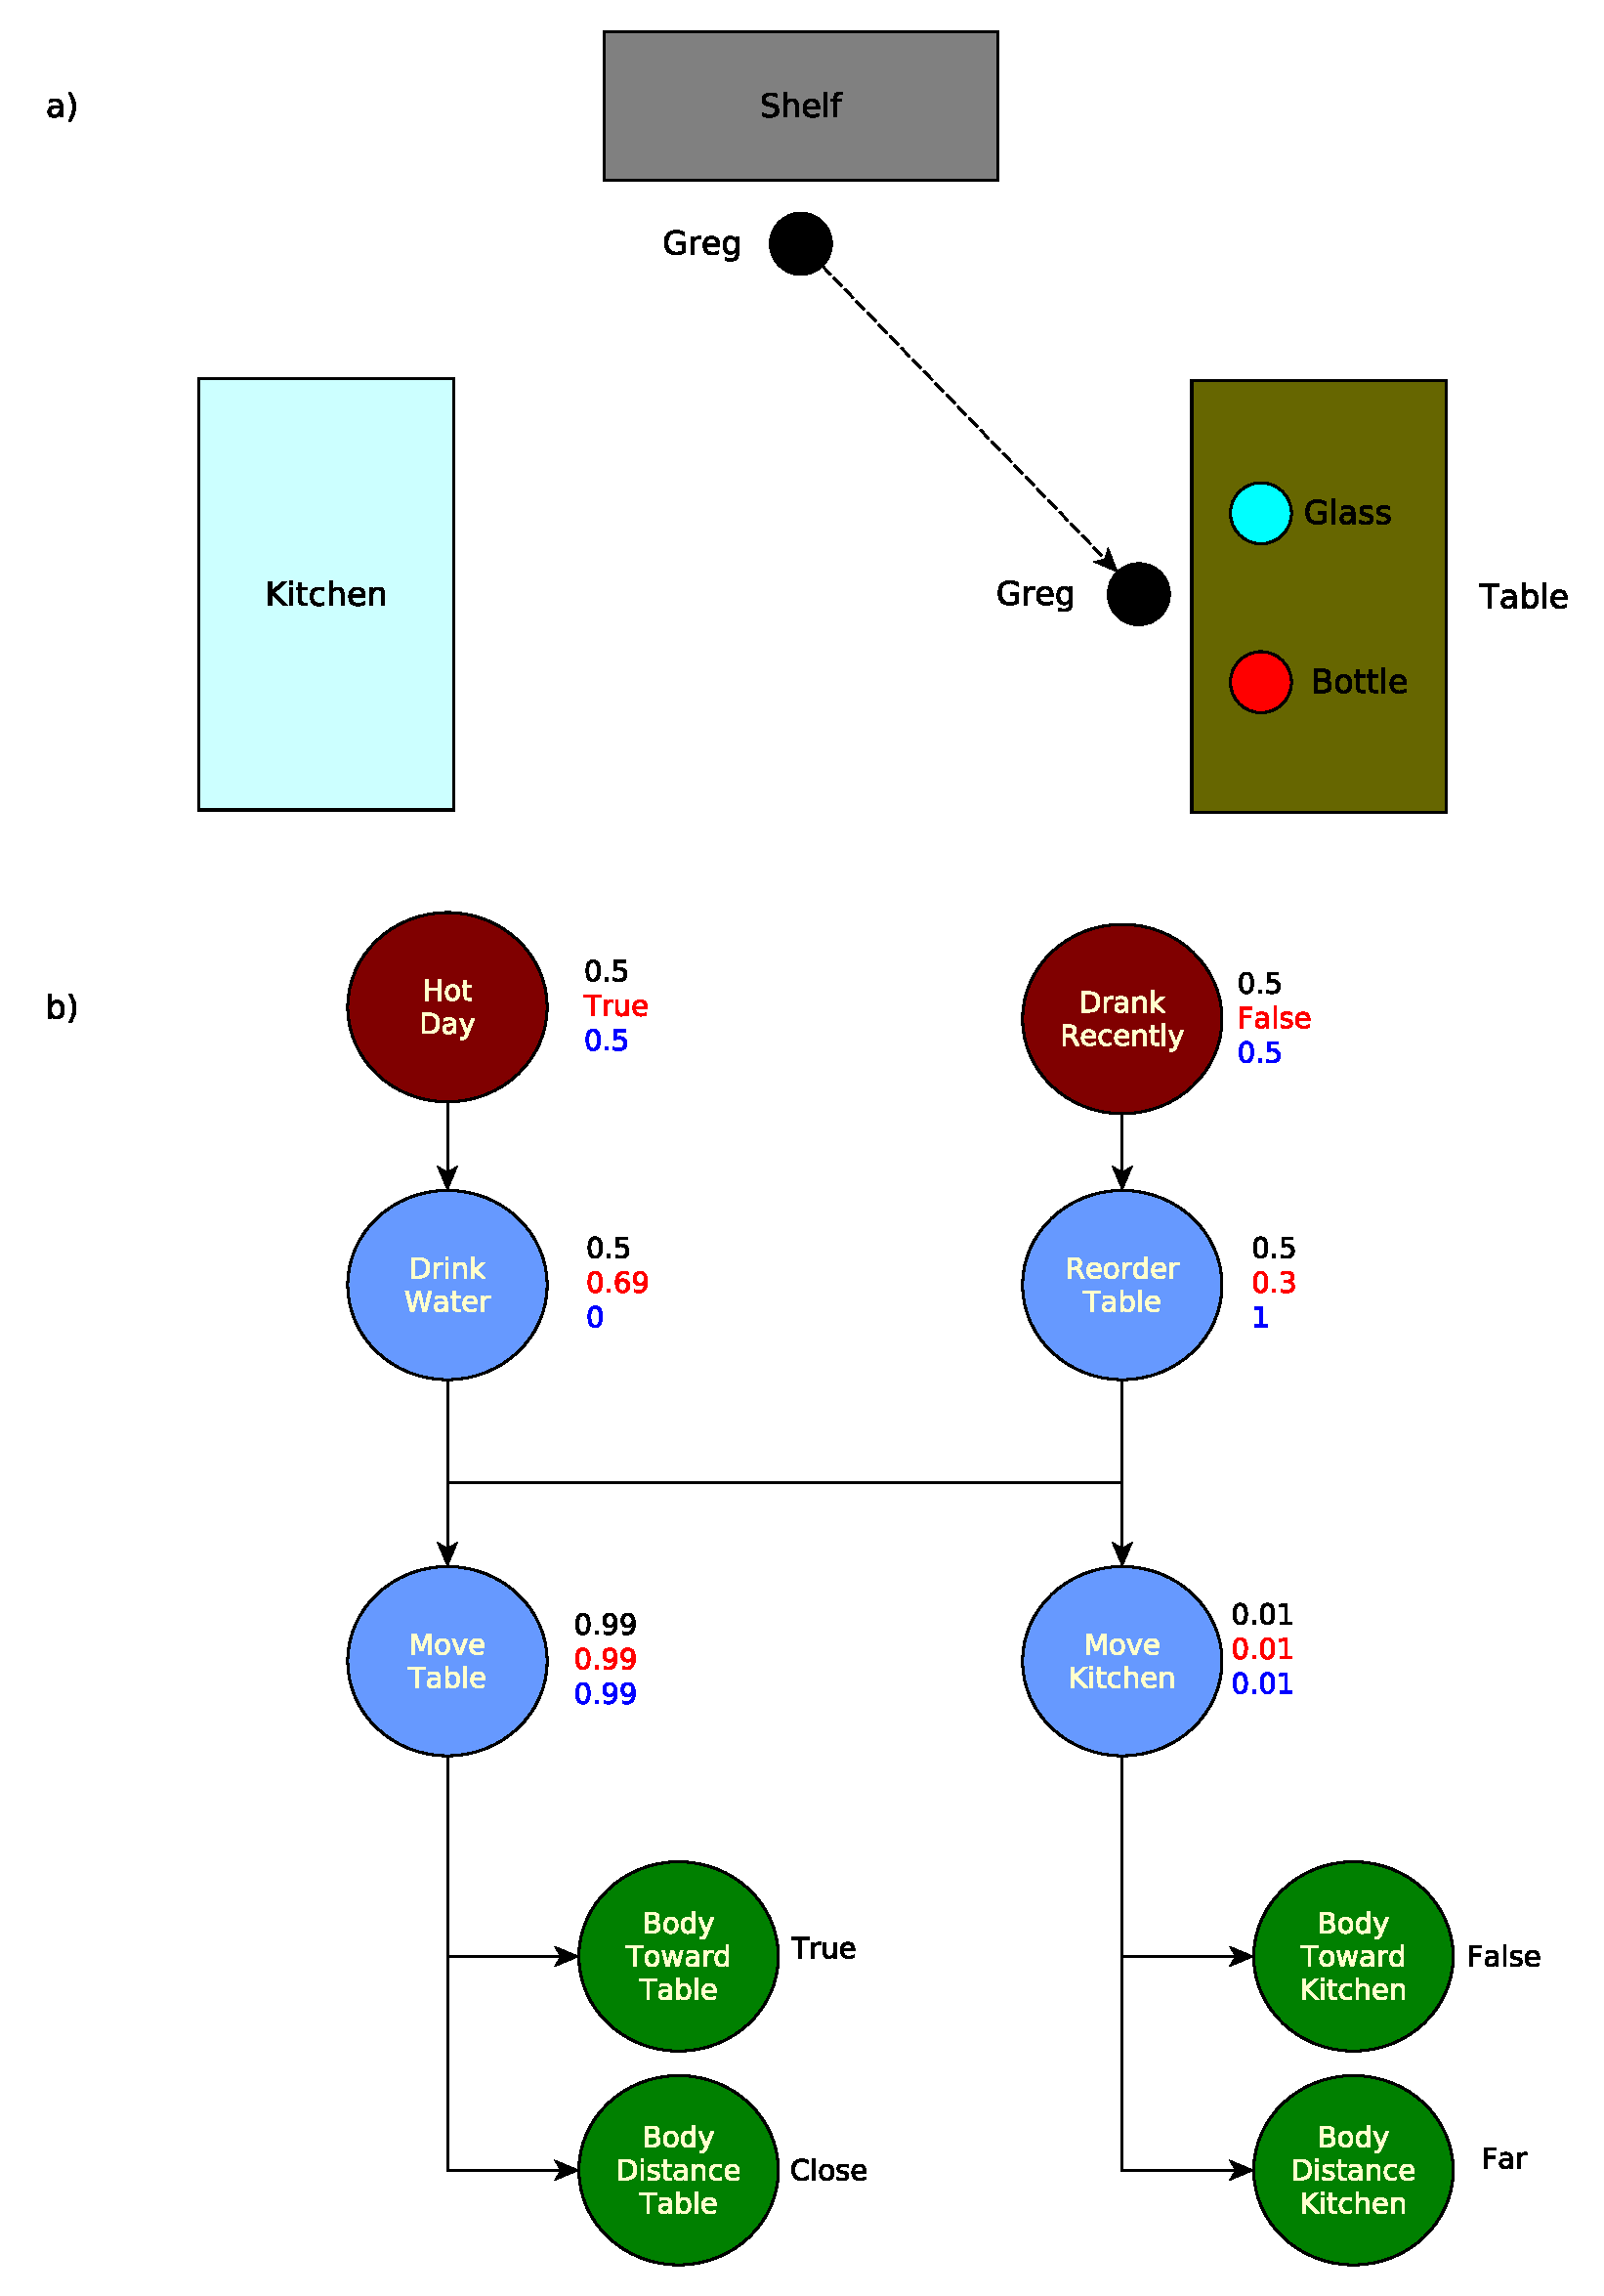
\includegraphics[scale=0.4]{img/observer/ig_exp1.pdf}
	\caption[IG Example 1]{a) Greg, represented as a black circle, is approaching the table. The two black circles correspond to his starting and ending location, with the dotted arrow showing the direction of his movement. b) The corresponding IG graph. Nodes are represented as circles and causal links as arrows. Intention and Action Nodes are represented as blue. Observation Nodes are represented as green to show that we consider them as evidence, fixing their values. Context Nodes are represented as red to mean that in the first and third test they are treated as standard nodes, and in the second as evidence.
 	 For each node we show the probability that its value is true or its current value, if the node is treated as evidence. We show three different values for each node: the black one shows the value if we compute the probability by using the human's mental belief (test 1), the red if we use the human's mental belief and treat Context Nodes as evidence (test 2), and the blue if we do not use context and use the robot's mental belief for the computation (test 3). Test 1 shows that at this point the system is not able to disambiguate between the two intention, which have a value of 0.50. Test 2 shows that context would help the robot to infer correctly the intention. Test 3 shows that by not using the human's mental belief the robot would discard the drink water intention, considering it not achievable.}
	\label{fig:intention-ig_exp1}
\end{figure}

\clearpage

\hfill
 \begin{figure}[ht!]
	\centering
	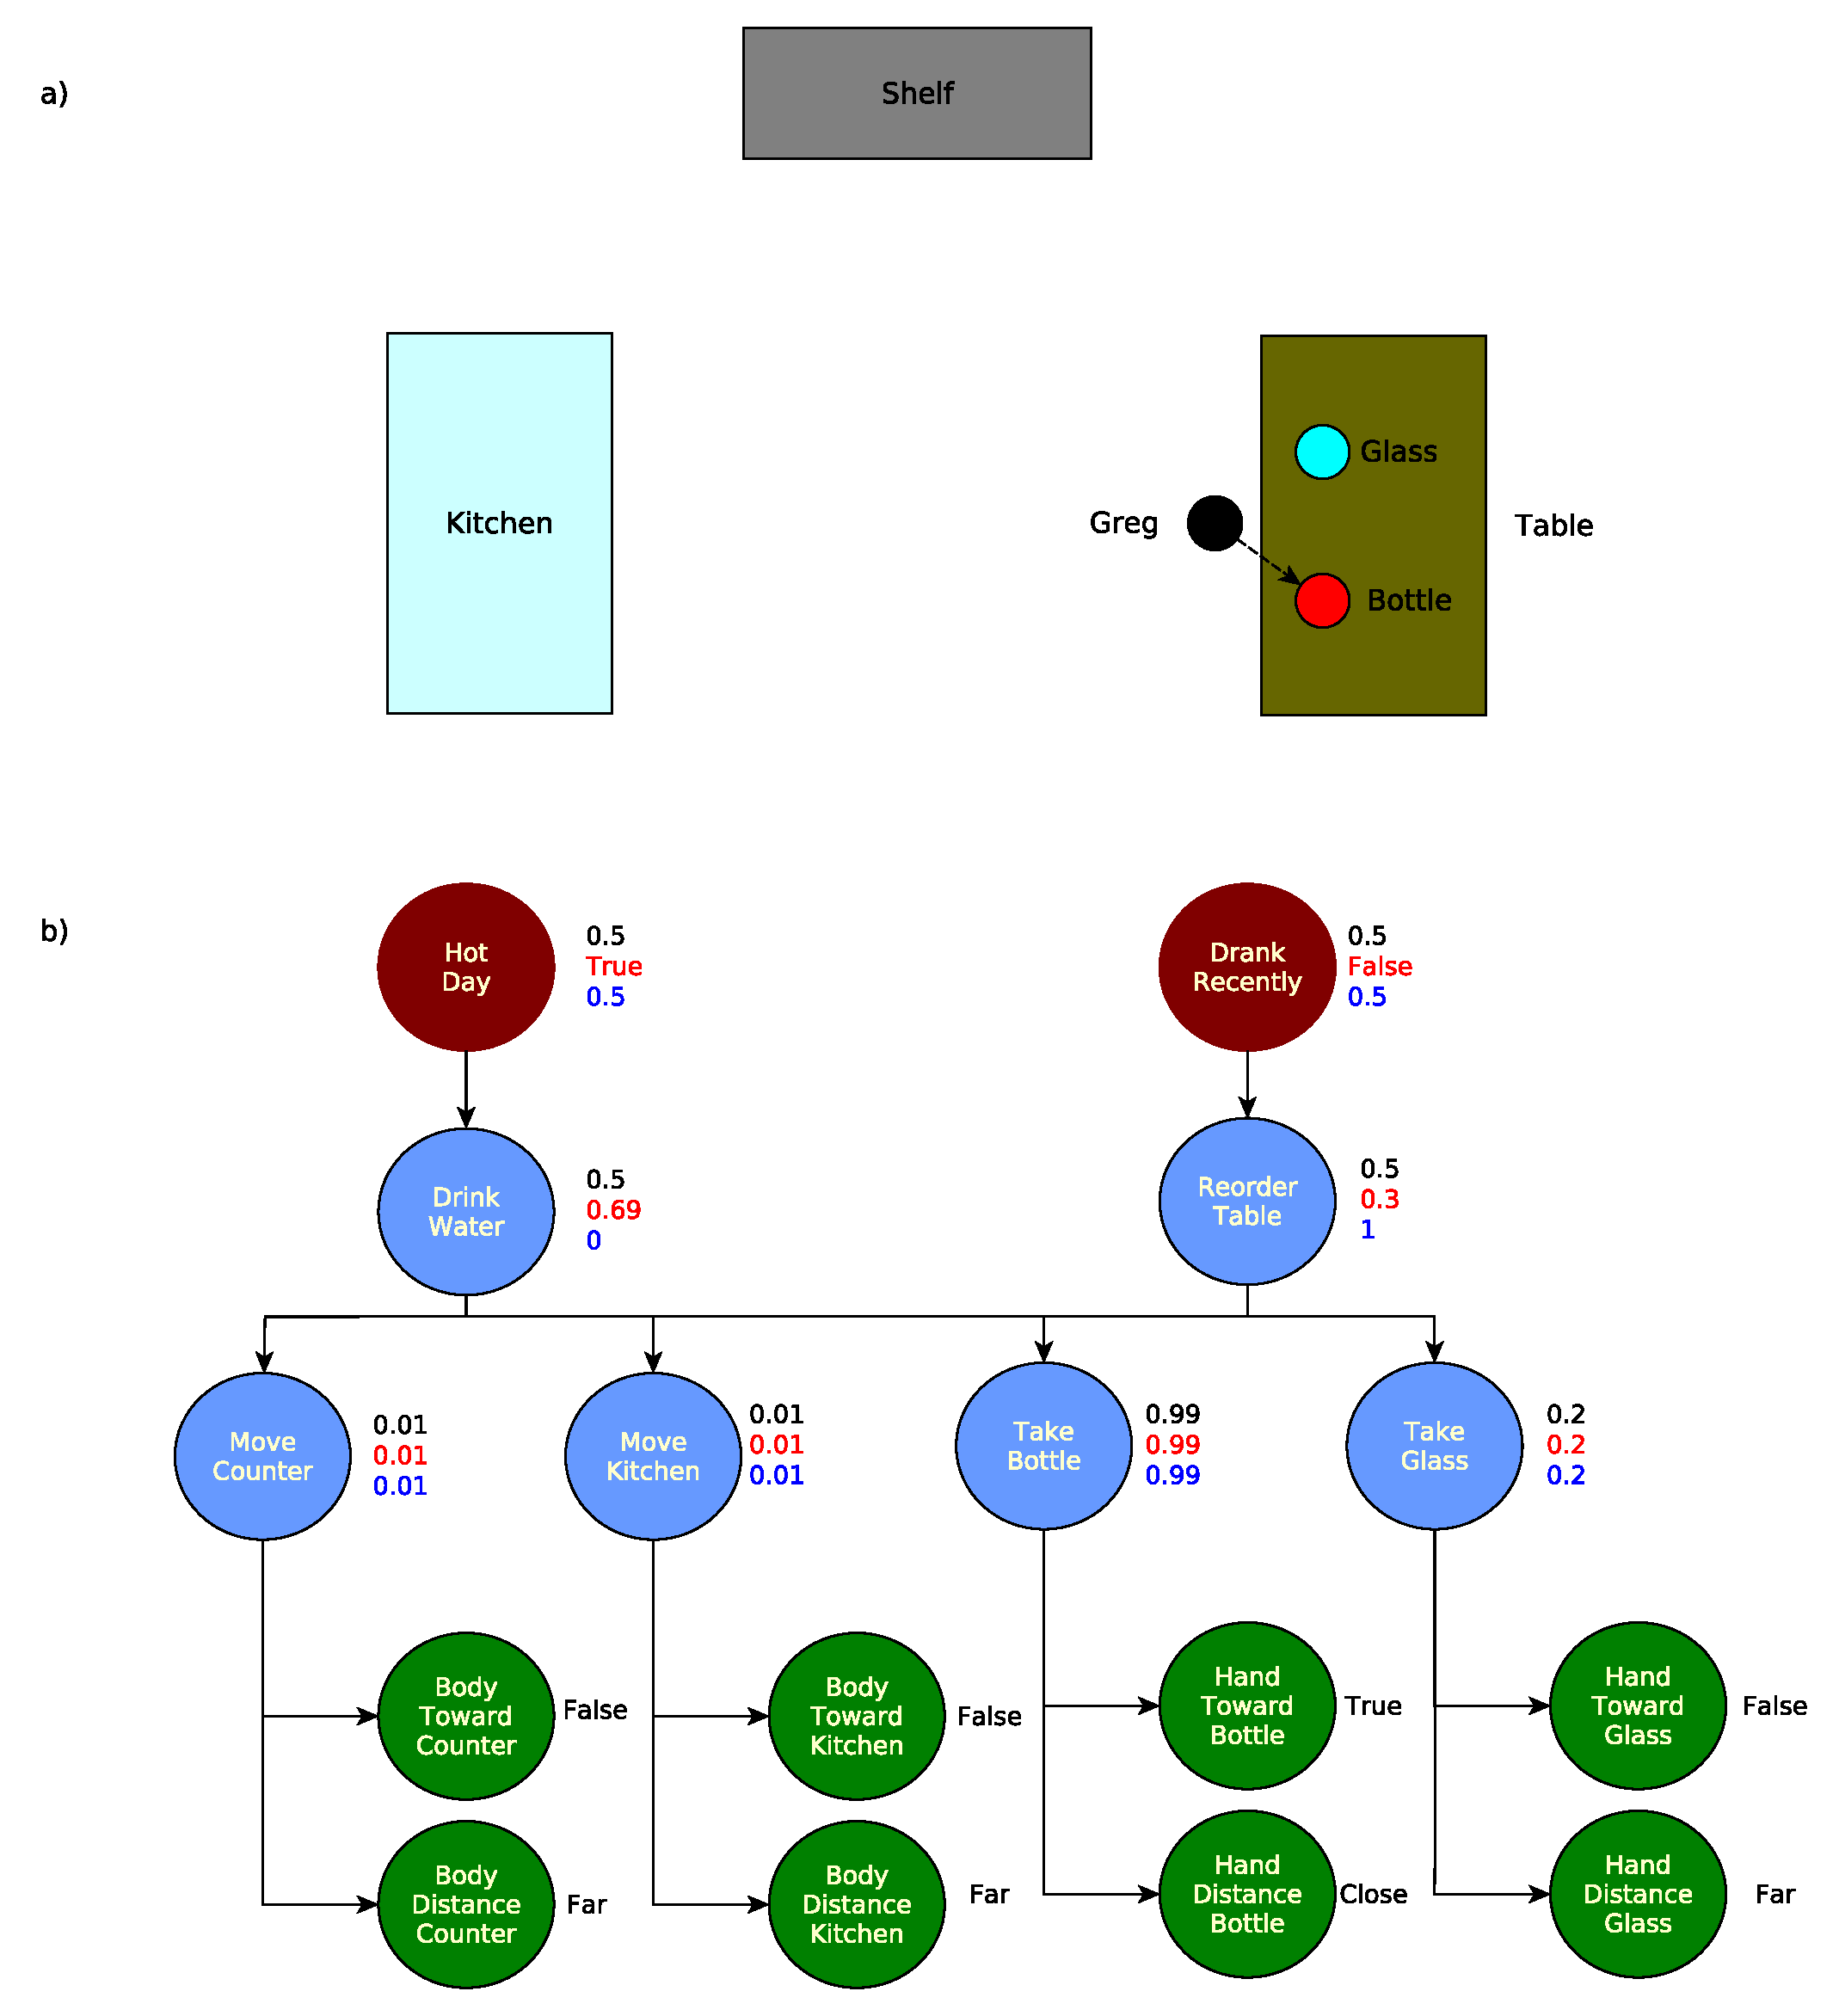
\includegraphics[scale=0.4]{img/observer/ig_exp2.pdf}
	\caption[IG Example 2]{a) Greg's hand is approaching the bottle. b) The corresponding IG graph. As before, test 1 is shown in black, test 2 in red, and test 3 in blue. The results of 
	the test are very similar to the previous time step, shown in figure~\ref{fig:intention-ig_exp1}.}
	\label{fig:intention-ig_exp2}
\end{figure}

\clearpage
 \begin{figure}[ht!]
	\centering
	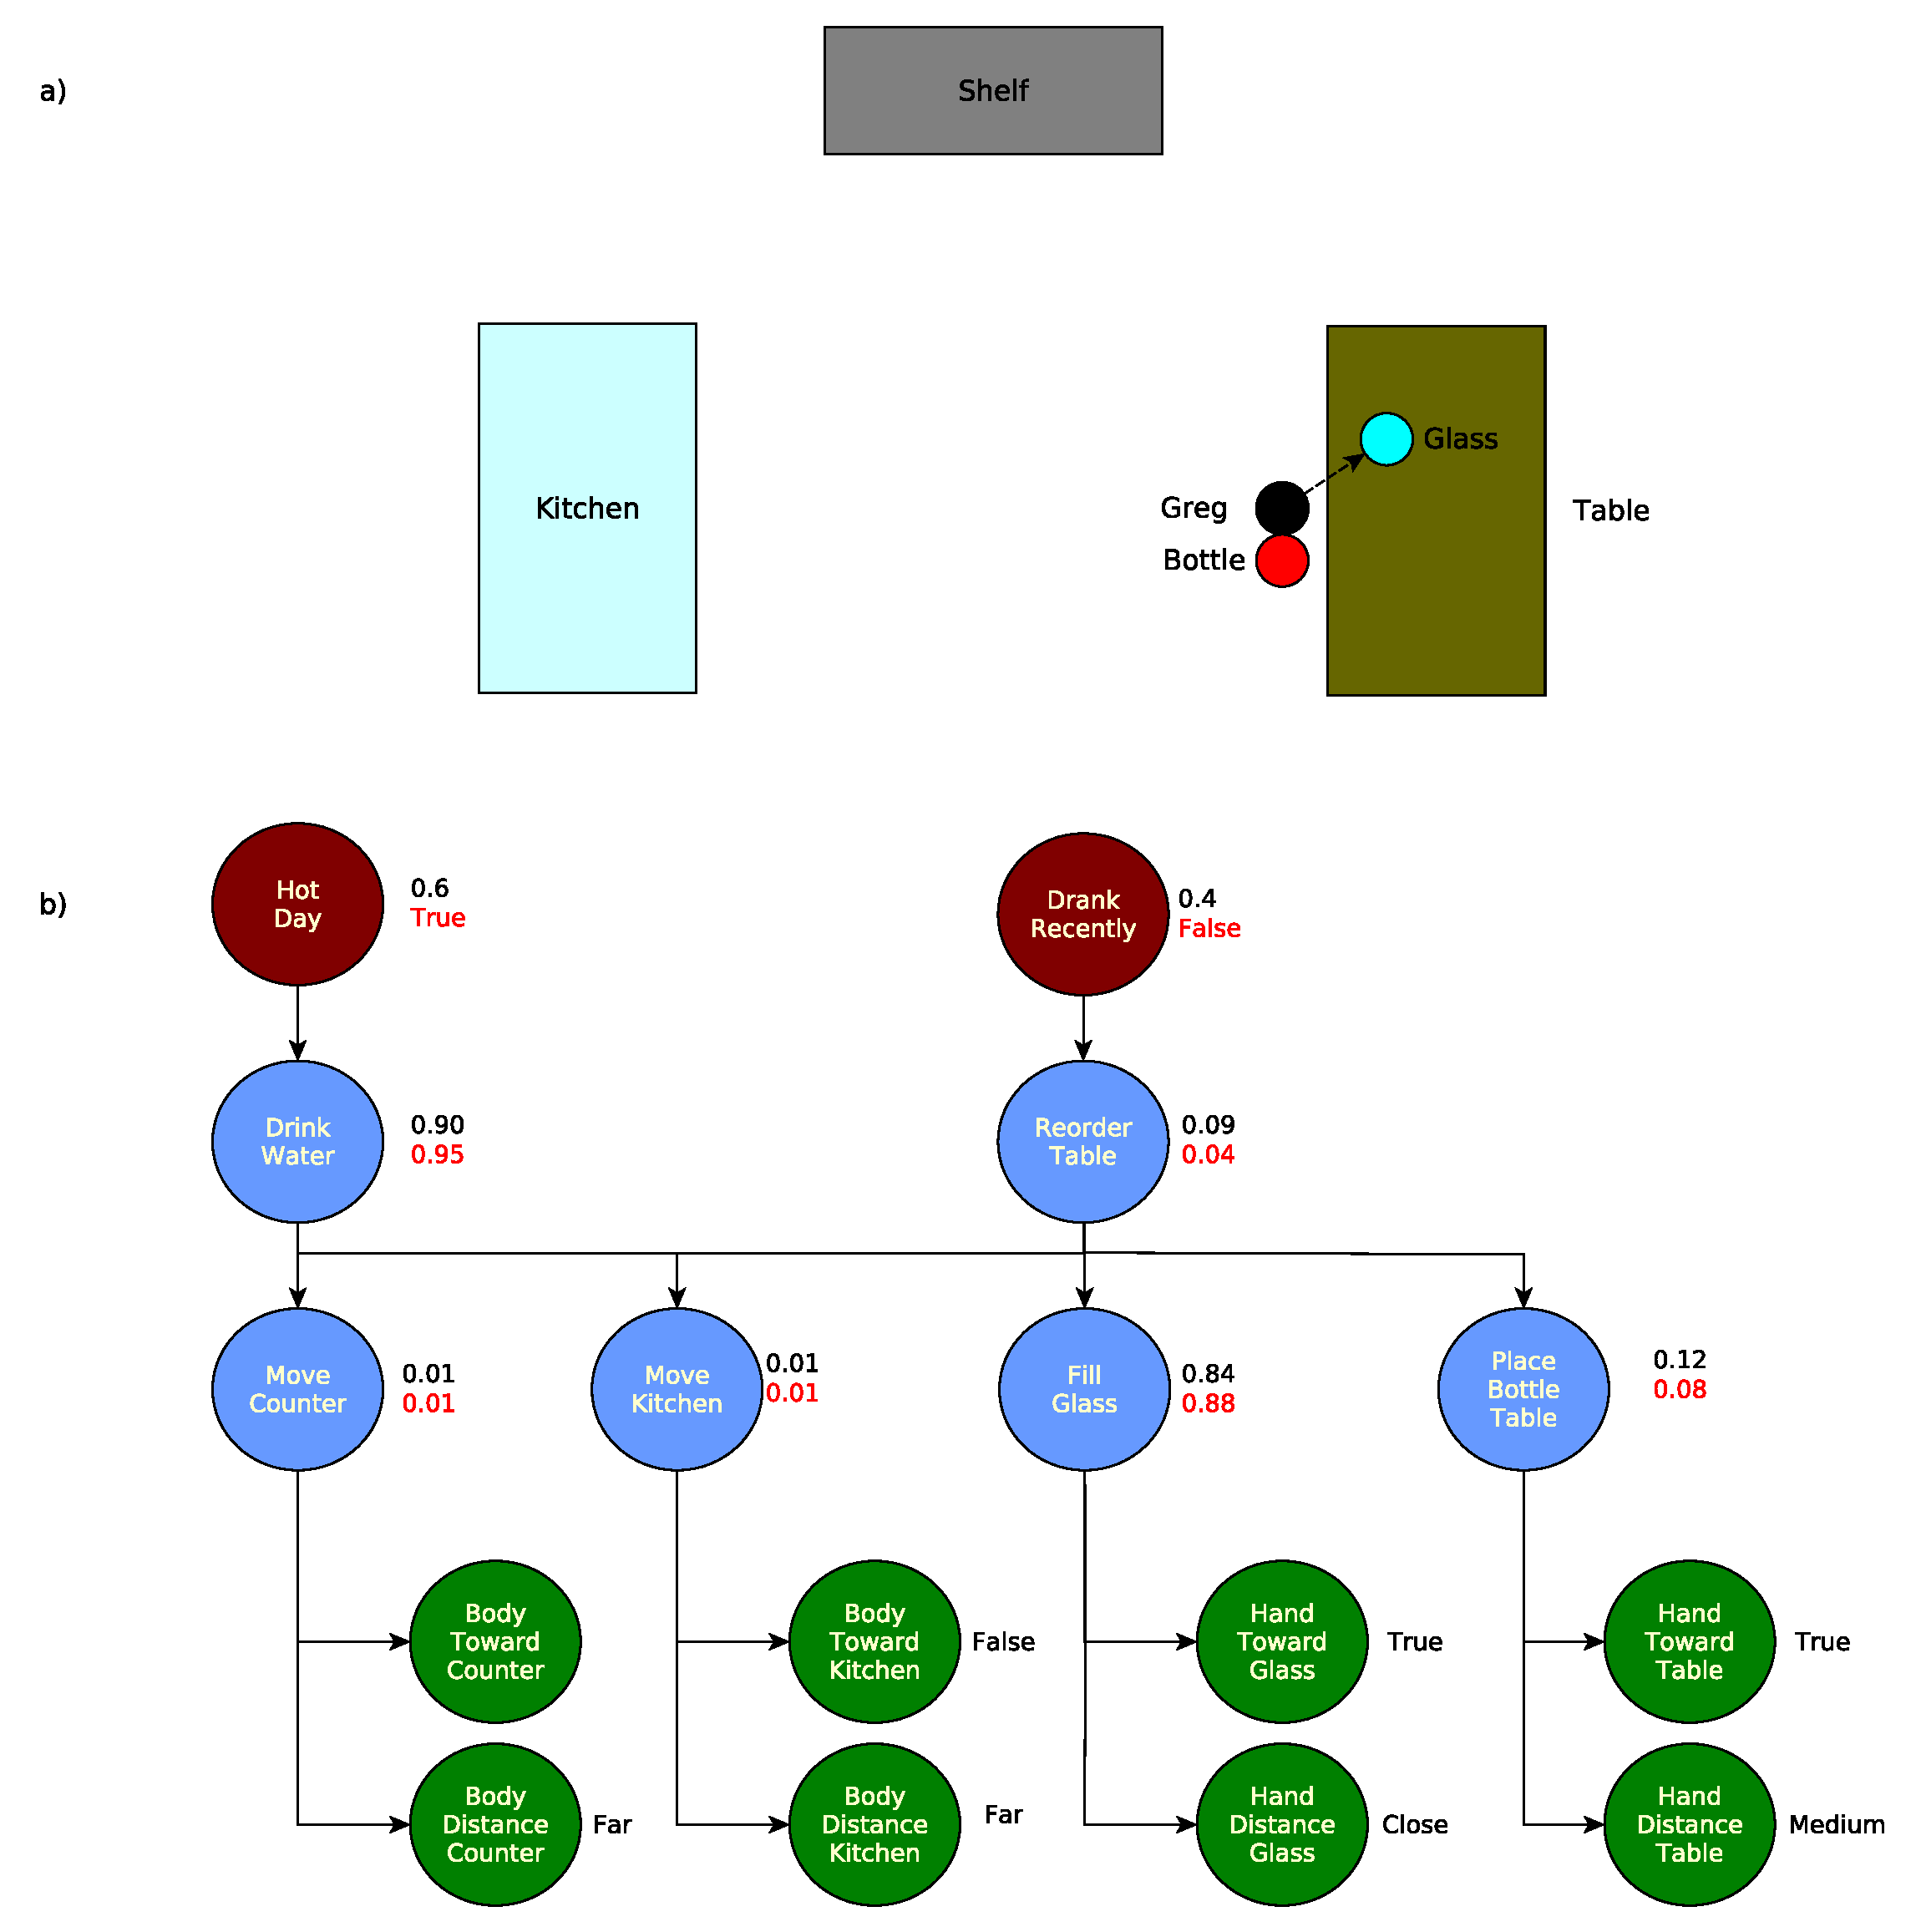
\includegraphics[scale=0.4]{img/observer/ig_exp3.pdf}
	\caption[IG Example 3]{a) Greg has taken the bottle, shown by placing the red circle and black circle close. His hand, with the bottle, is now approaching the glass b) The corresponding IG graph. As before, test 1 is shown in black and test 2 in red. Test 3 is not shown since the fill glass action would not be executable in the robot's mental belief model, and so the corresponding IG would be different. In test 1 the system has now sufficient information to infer the correct intention, which has a value of 0.90. Test 2 confirms this choice.}
	\label{fig:intention-ig_exp3}
\end{figure}
\clearpage

\section{Discussion}

This component is able to estimate the likelihood of a human's intention by combining BNs, MDPs, geometrical reasoning, and the capacity to model human's beliefs. Contextual information can further help to disambiguate the inference process. 

Another advantage of our approach is its good scalability. Computing the probabilities in a BN can be done using efficient and well know algorithms, which scale well with the size of the network, meaning that the IG is able to accomodate the addition of new actions, observations and contexts. 

Adding a new intention means creating and solving another MDP. Since this process is done offline this would not impact the run of the system. When computing the conditional probabilities of the action nodes, the system uses the action value function of the MDPs, which is stored in memory and can be directly accessed.
